\documentclass[a4paper, 12pt]{ctexart}
\usepackage{amsmath}
\usepackage{graphicx}
\title{FFT仿真报告}
\author{吴彦成}
\date{\today}

\begin{document}
\maketitle
\section{概述}
本次仿真的最终目标是在matlab中完成实现一个64位的FFT的运算的函数。该函数的输入是$1 \times 64$的向量,输出是$1 \times 64$的向量。相较于DFT算法,该算法可以将乘法的使用次数从$64^2$降低到$64 \times 8$。

该算法的核心思想是运用原文中的公式(3):

\begin{equation*}
    \begin{aligned}
        F(k) &= \sum_{n = 0}^{63} x(n)W_{64}^{nk}\\
        &= \sum_{n_2 = 0}^{7} W_{8}^{n_2k_1}[W_{64}^{n_2k_2} \sum_{n_1 = 0}^{7} x(8n_1 + n_2)W_8^{n_1k_2}]\\
    \end{aligned}
\end{equation*}

其中,$F(k)$是FFT输出的64位向量的第$k$项,$x$是FFT输入的64位原始数据向量,$W_N = e^{-2 \pi i / n}$.

公式(3)利用三角函数的周期性,将公式第一行的64次运算简化为了第二行的16次运算。在后续的操作中,我们会进一步利用此特性将16次运算简化到8次。

\section{进一步化简以及对公式错误的修正}

为了实现进一步的化简,我们注意到形如:
$$\sum_{m = 0}^{7} x(m)W_8^{mk}$$
的结构多次出现。

在原文公式(4)中也对此结构进行了描述,但有一些符号上的错误,具体如下:
\begin{figure}[h]
    \centering
    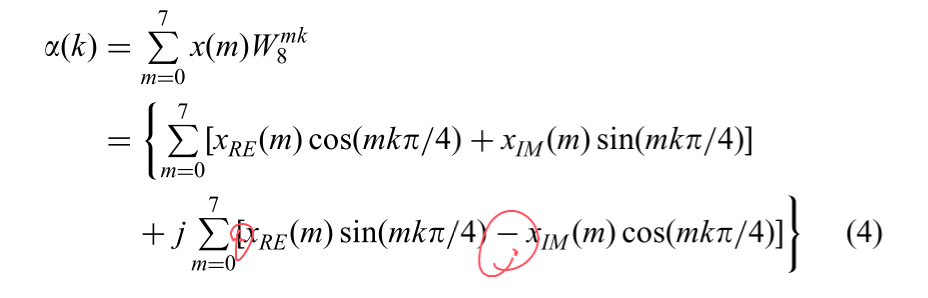
\includegraphics[width=0.8\linewidth]{4.png}
\end{figure}

我们对其修正如下:

\begin{equation*}
    \begin{aligned}
        \alpha(k) &= \sum_{m=0}^7 x(m)W^{mk}\\
        &= \sum_{m=0}^7 [x_{RE}(m)cos(\frac{mk \pi}{4}) + x_{IM}(m)sin(\frac{mk \pi}{4})]\\
        &+j \sum_{m=0}^7 [-x_{RE}(m)sin(\frac{mk \pi}{4}) + x_{IM}(m)cos(\frac{mk \pi}{4})]
    \end{aligned}
\end{equation*}

利用三角函数的基本性质:
\begin{figure}[h]
    \centering
    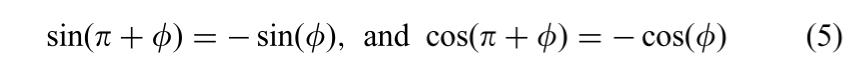
\includegraphics[width=0.8\linewidth]{5.png}
\end{figure}

文中对公式(4)进行了如下的进一步化简:
\begin{figure}[h]
    \centering
    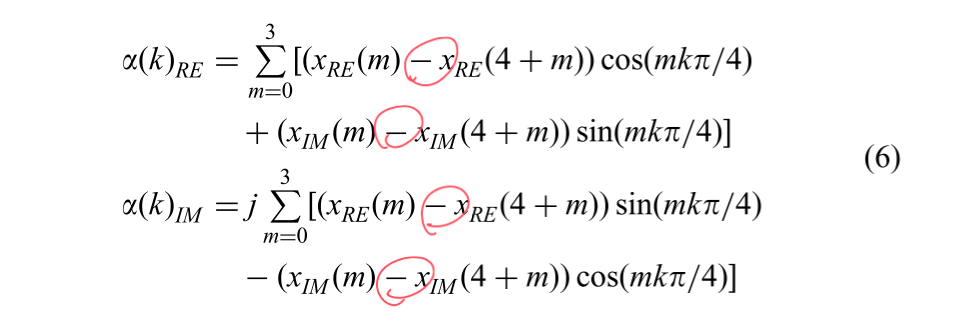
\includegraphics[width=0.8\linewidth]{6.png}
\end{figure}

此番操作是在公式(4)错误的基础上再误认为$cos((4 + m)k \pi / 4) = -cos(mk \pi / 4)$对一切的$k$都成立。然而事实上,$cos((4 + m)k \pi / 4) = cos(mk \pi / 4 + k \pi) = (-1)^k cos(mk \pi / 4)$。我们对公式(6)修正如下:

\begin{equation*}
    \begin{aligned}
        \alpha(k)_{RE} &= \sum_{m=0}^3 [(x_{RE}(m) + (-1)^k x_{RE}(4 + m))cos(\frac{mk \pi}{4})\\
        &+(x_{IM}(m) + (-1)^k x_{IM}(4 + m))sin(\frac{mk \pi}{4})]
    \end{aligned}
\end{equation*}

\begin{equation*}
    \begin{aligned}
        \alpha(k)_{IM} &= j\sum_{m=0}^3[-(x_{RE}(m) + (-1)^k x_{RE}(4 + m))sin(\frac{mk \pi}{4})\\
        &+ (x_{IM}(m) +(-1)^k x_{IM}(4 + m))cos(\frac{mk \pi}{4})]
    \end{aligned}
\end{equation*}

通过修正后的$\alpha$操作,我们将需要的乘法次数从原来的8次缩减到现在的4次。

\section{仿真的流程}

我们注意到在公式(3)中括号内的部分:
$$W_{64}^{n_2k_2} \sum_{n_1 = 0}^{7} x(8n_1 + n_2)W_8^{n_1k_2}$$
只与$n_2$和$k_2$有关,并且当$n_2$和$k_2$遍历$0 \sim 7$时,其也会遍历64个值,所以也可以把这一部分看作一个64位的中间向量。我们仿真的第一步就是要得到这个中间向量。

得到中间向量的方法其实就是遍历$n_2$和$k_2$,对每一个确定的$n_2$和$k_2$通过上述公式计算对应的值。当然,对于
$$\sum_{n_1 = 0}^{7} x(8n_1 + n_2)W_8^{n_1k_2}$$
我们可以利用之前讨论过的$\alpha$操作将循环的次数从8次降到4次。这样一来,我们便顺利地得到了中间向量$y$。

下一步我们便可以直接通过中间向量$y$得到最终的结果:
$$F(k) = \sum_{n2 = 0}^{7} W_8^{n_2k_1} y(8k_2 + n_2)$$
注意到这一部分的和只与$k_1$和$k_2$有关,并且这样的结构同样可以使用$\alpha$操作将循环的次数从8次降到4次。

至此我们便顺利得到了FFT的结果,一个64位的向量。

\section{误差分析}

为了验证仿真的正确性,我们用均方根进行了误差估计。具体的操作是每次生成一组64位随机数组成的向量作为函数的输入,将得到的结果与matlab内置的FFT得到的结果进行均方差估计,并重复1000次,最终结果如下:
\begin{figure}[h]
    \centering
    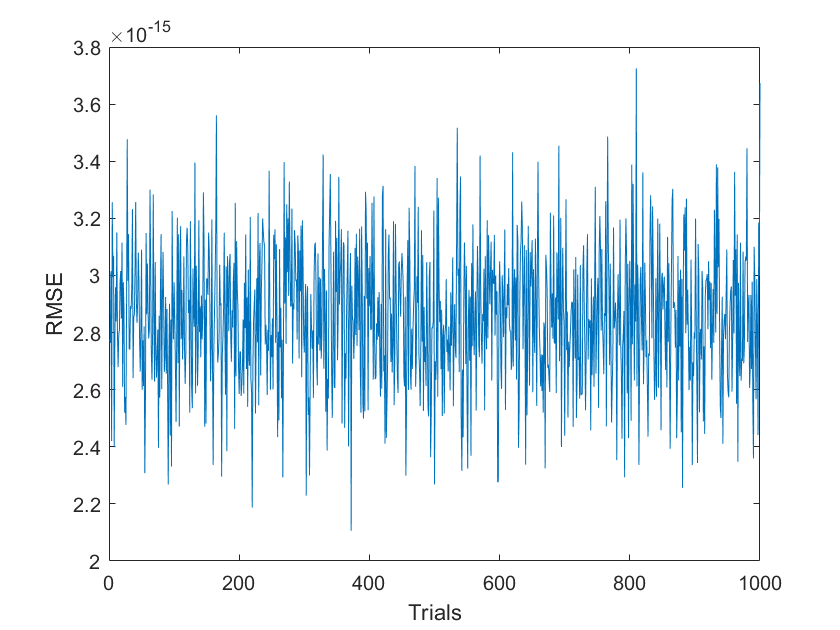
\includegraphics[width=0.8\linewidth]{error.png}
\end{figure}

如果将1000组64位随机向量视为一组64000位的数据,其最终的均方根误差为$2.8628 \times 10^{-15}$。误差在可接受范围之类。

\section{总结}

本次仿真成功地完成了对原文中除去LUTs以外核心算法的论证,为下一步工作奠定了基础。

\end{document}